%!TEX root = main.tex
\section{Results}
\subsection{With and without Olympic Games}
Choosing $\beta=2$, $\gamma=0.5$ and an average transfer probability of $0.005$ we can run a simulation with and without the Olympic Games occurring with the previously described characteristics. We assume that the infection breaks out on the first day of the games in Rio De Janeiro. We set the initial infected population to 1000. In the following we will look at the SIR curves of 6 major cities.

With the Olympics occurring we get the following curves:
\begin{figure}[H]
	\centering
	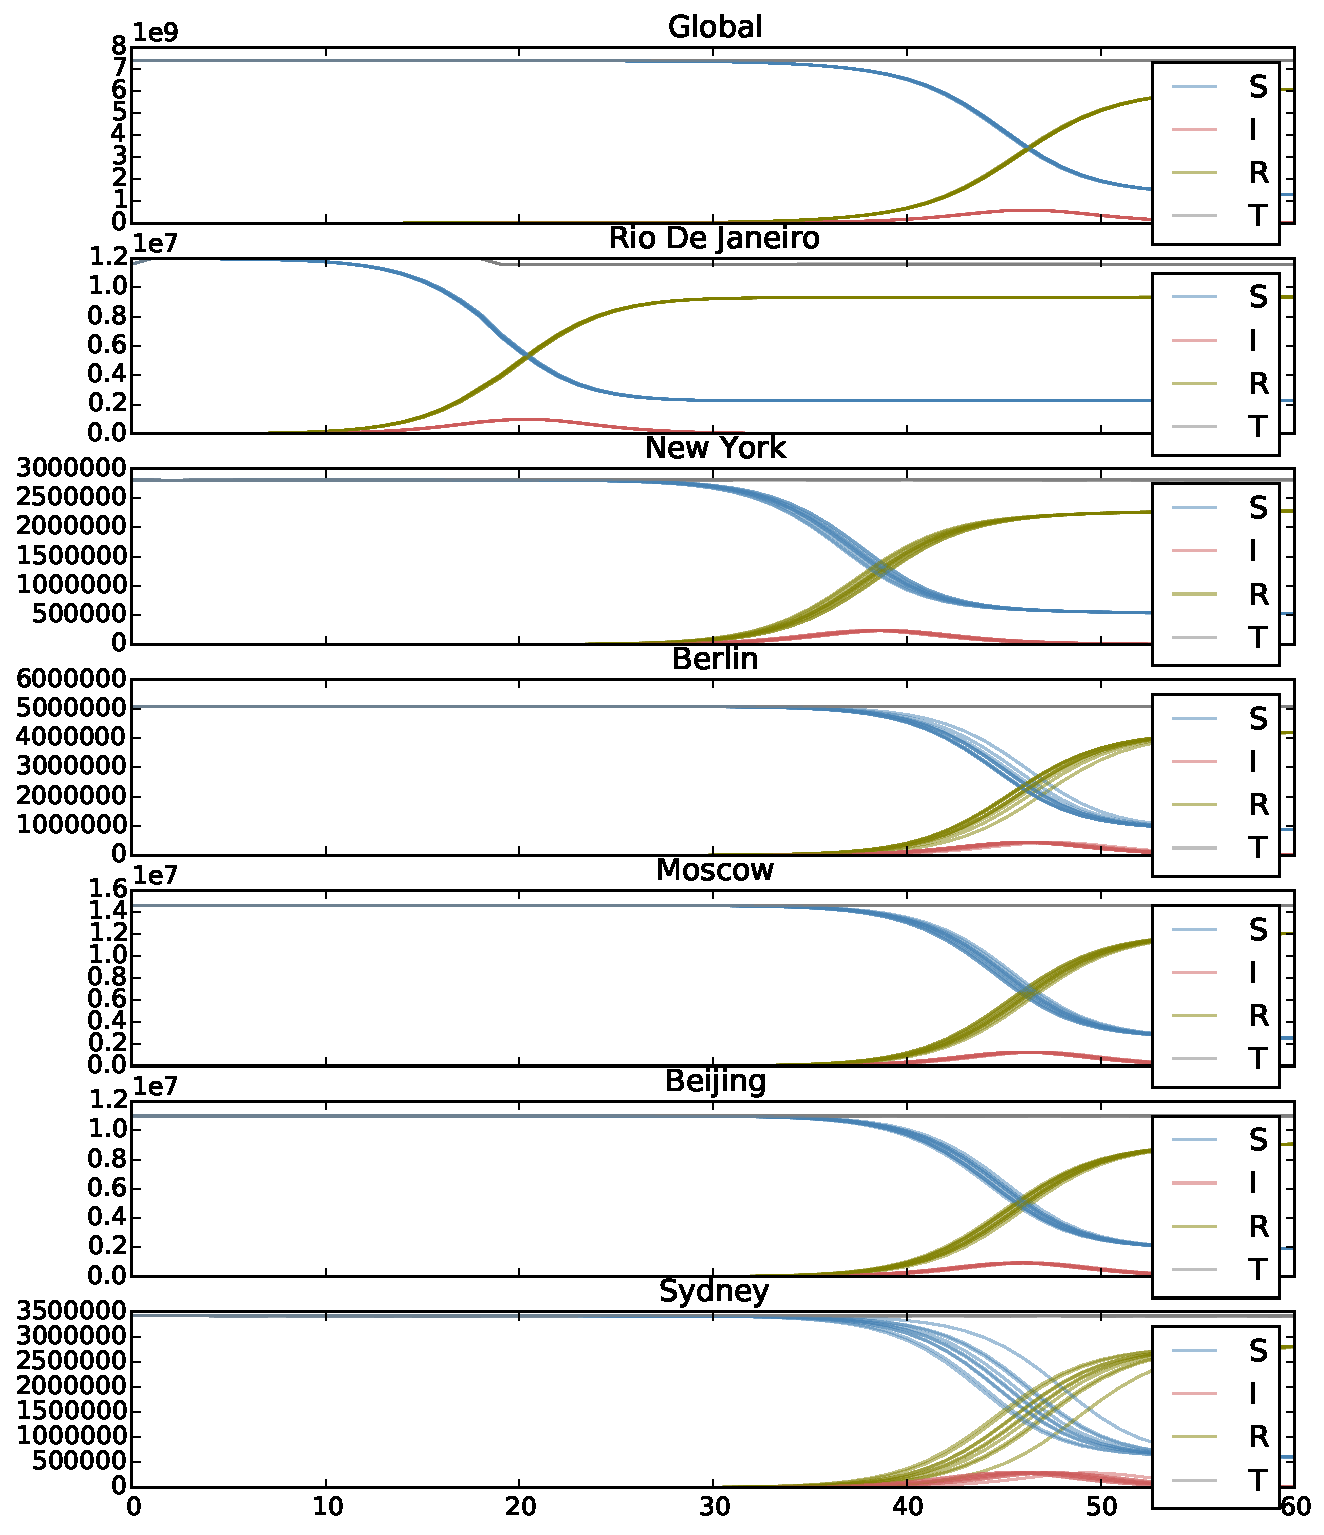
\includegraphics[width=1.0 \linewidth]{plots/rio-0-18-380000.pdf}
	\caption{10 simulations with Olympic Games. Time in days on the x-axis and number of people on the y-axis. Shown is susceptible (S), infected (I), removed (R) and total population (T).}
	\label{fig:rio-0-18-380000}
\end{figure}

From figure \ref{fig:rio-0-18-380000} it's seen that except for Rio where the infection started and New York which seems to be infected earliest, the other major cities all seem to reach peak infection rates at approximately the same time. 

\begin{figure}[H]
	\centering
	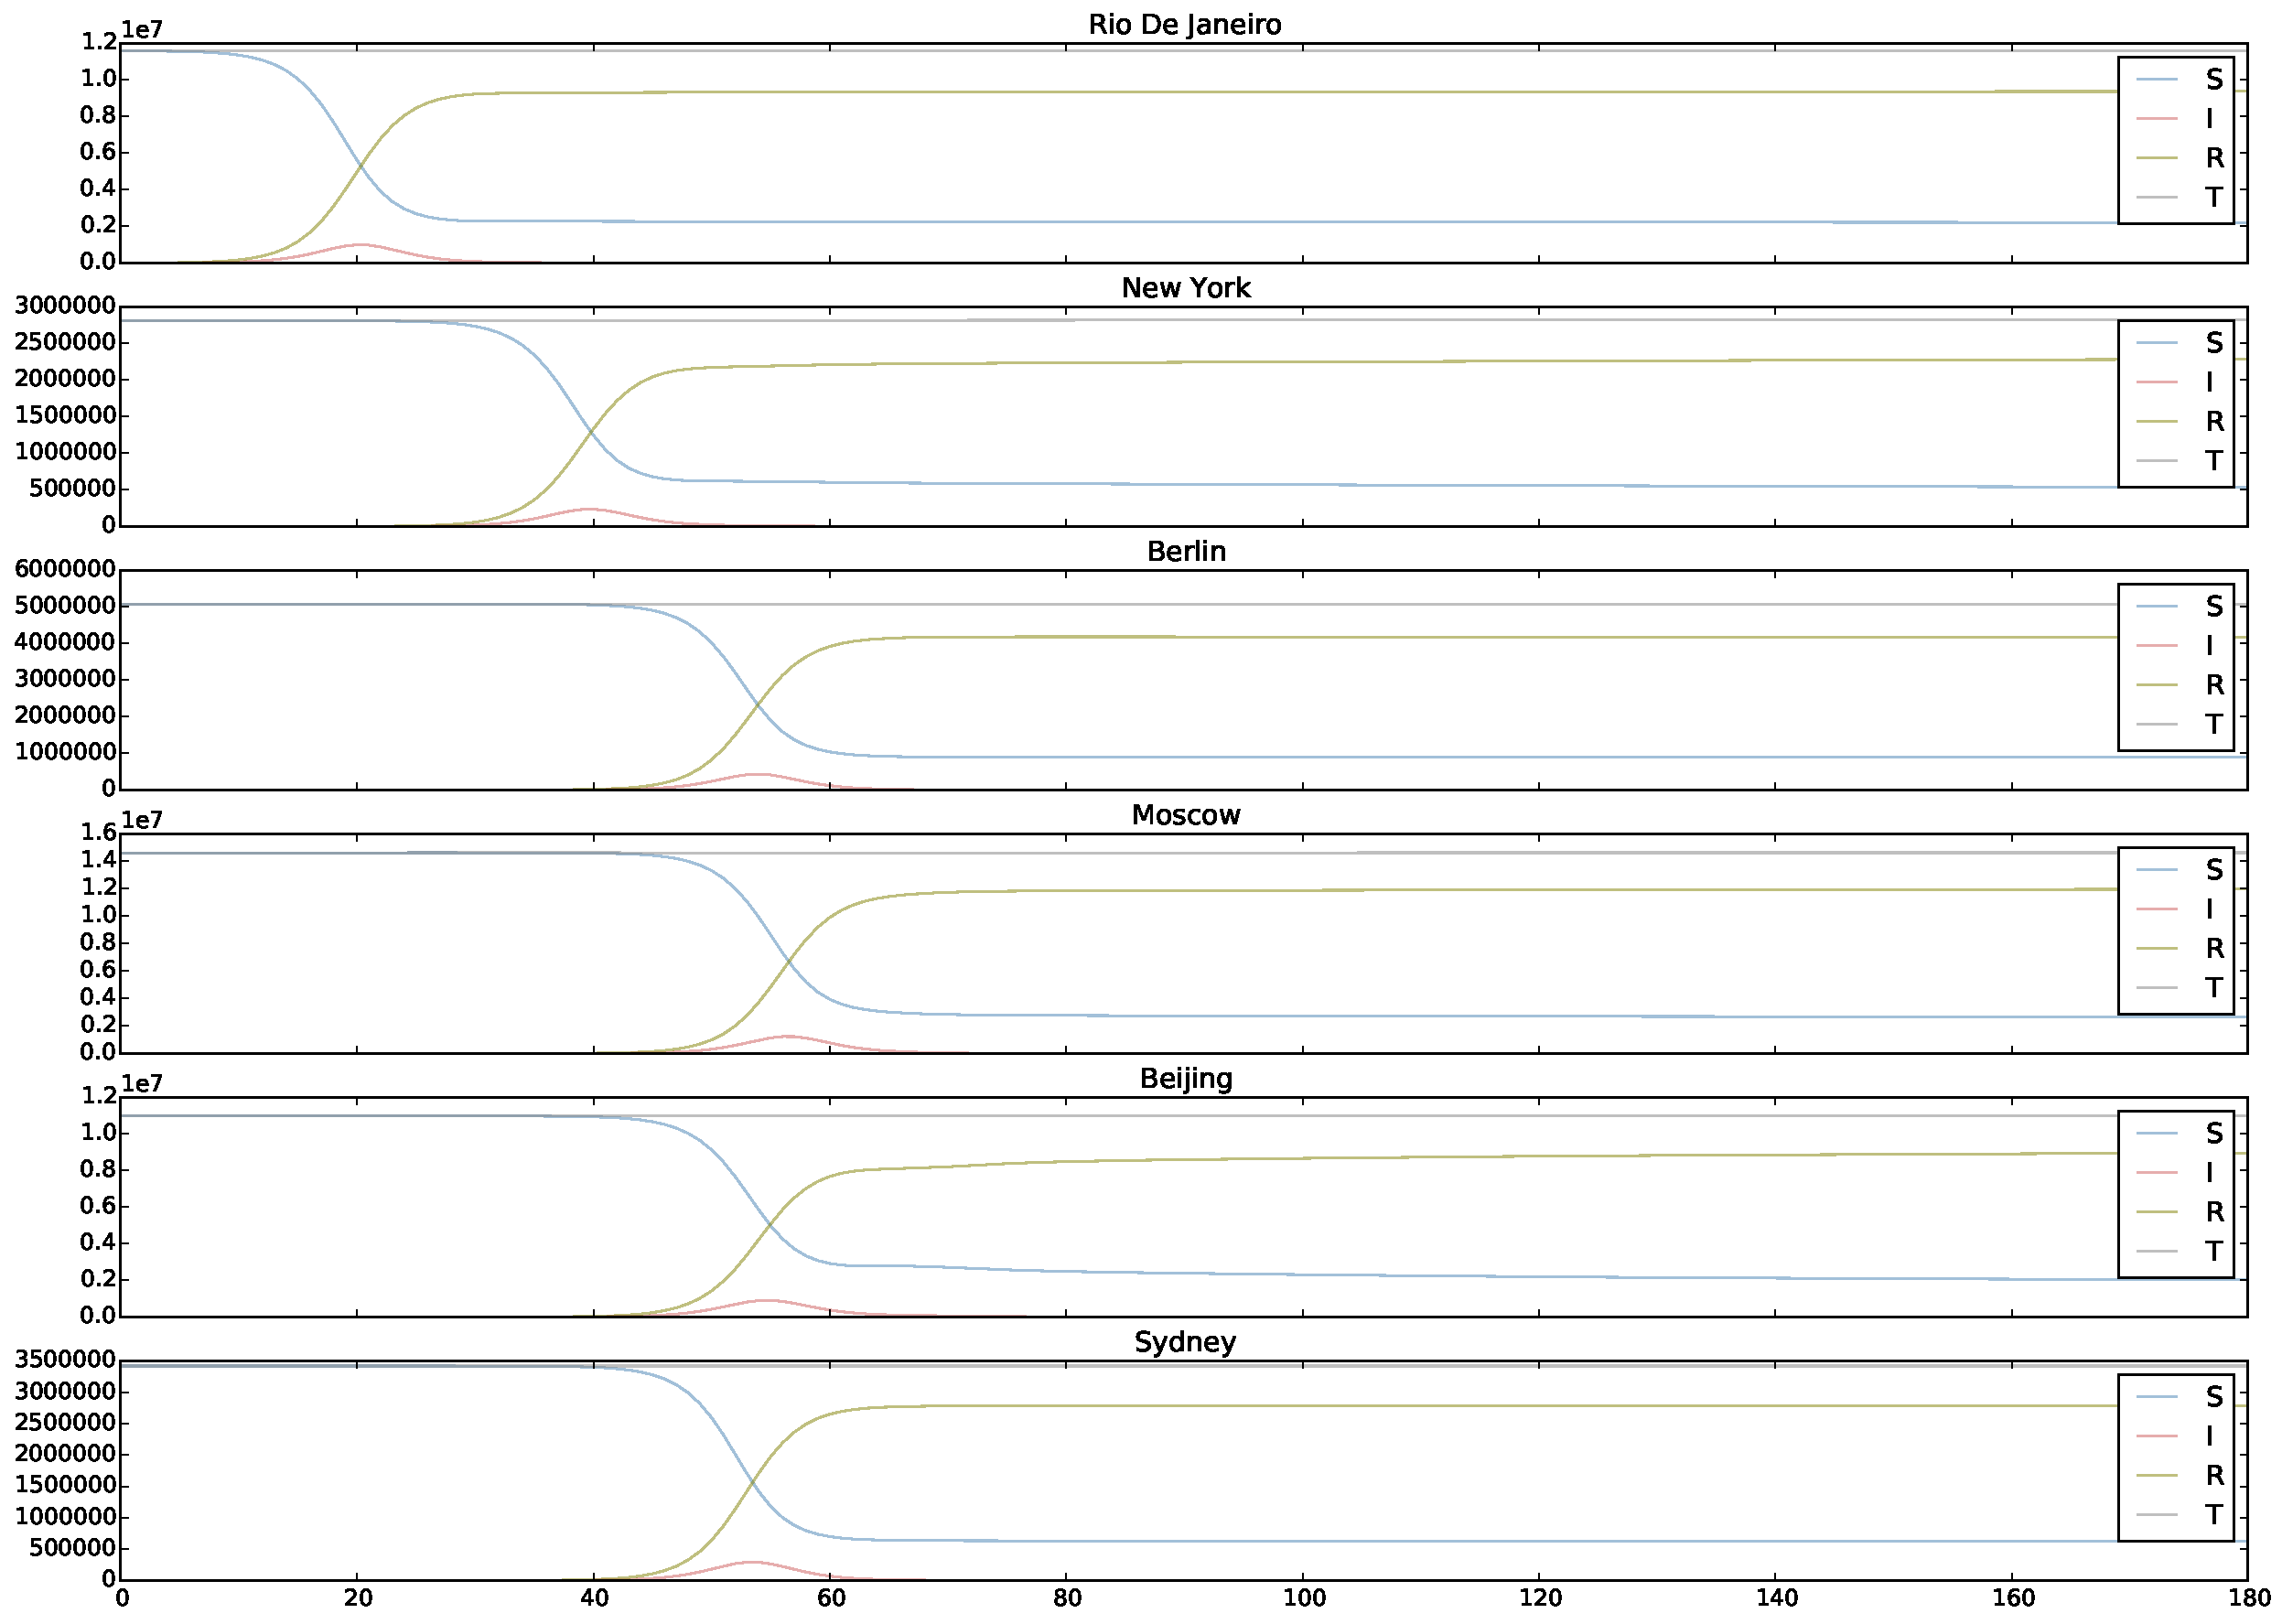
\includegraphics[width=1.0 \linewidth]{plots/no_rio.pdf}
	\caption{10 simulations without Olympic Games. Time in days on the x-axis and number of people on the y-axis. Shown is susceptible (S), infected (I), removed (R) and total population (T).}
	\label{fig:no_rio}
\end{figure}

When there is no Olympic Games, as seen in figure \ref{fig:no_rio}, the peak infections occur later, especially for Moscow, Beijing and Sydney. The is emphasized in the summary table \ref{table:olympic-summary}.

\begin{table}[H]
	\centering
	\begin{tabular}[H]{c | c | c}
Observation & With OL & Without OL \\ \hline 
 Peak amount Global [million]& $590.5\pm 0.94 (0.02)$ & $291.5 \pm 1.41 (0.01)$\\ 
 Peak time Global & $46.0\pm 0.00( 0.00)$ & $67.0 \pm 0.00 (0.00)$\\ 
 Peak time Rio & $20.2\pm 0.30( 0.26)$ & $20.0 \pm 0.00 (0.00)$\\ 
 Peak time New York & $38.6\pm 0.50( 0.52)$ & $38.3 \pm 0.59 (0.50)$\\ 
 Peak time Berlin & $46.4\pm 0.77( 0.56)$ & $53.7 \pm 0.35 (0.30)$\\ 
 Peak time Moscow & $46.1\pm 0.23( 0.23)$ & $56.3 \pm 0.35 (0.28)$\\ 
 Peak time Beijing & $46.0\pm 0.00( 0.00)$ & $55.0 \pm 0.34 (0.30)$\\ 
 Peak time Sydney & $46.3\pm 0.83( 0.73)$ & $53.3 \pm 0.48 (0.51)$
\end{tabular}
	\caption{Results of 10 simulations with and without Olympic Games. Table contains the peak times and amounts for the number of infected individuals. The standard $95\%$-confidence interval is marked with $\pm$ and the confidence interval using control variates is shown in the parenthesis.}
	\label{table:olympic-summary}
\end{table}

As mentioned in table \ref{table:olympic-summary} one can see that when the Olympic Games occur the peak time is much less spread and generally happens earlier. This is particularly apparent when comparing with the global peak time, which in the case without Olympic Games, happens statistically significantly later when comparing to the cities. However, in the Olympic Games case, the city peak times are not statistical different from the global peak time (except for the New York and Rio).

The fact that Rio doesn't have a significantly difference in peak time makes sense because this is where the infection starts. Adding 380000 people (out of 12 million people) doesn't make much of a difference. The New York case is also interesting as there isn't a significant change. This is likely because New York being in north America and Rio being in South America is much more closely connected through airlines, compared to cities which are across the Pacific or Atlantic Ocean.

Finally table \ref{table:olympic-summary} also shows that the number of people infected globally is almost twice as big when including the Olympic Games compared to not including the Olympic Games.

Finally table \ref{table:olympic-summary} also shows that the number of people infected globally is almost twice as big when including the Olympic Games compared to not including the Olympic Games.

\subsection{Visualization of result}
When studying a virus outbreak it is interesting to see exactly how the virus spreads. We have thus created an animation on a world map showing where each region is represented as a dot. Each dot is placed at the region center (airport), scaled according to the population size, and the color represents the fraction infected.

\begin{figure}[H]
	\centering
	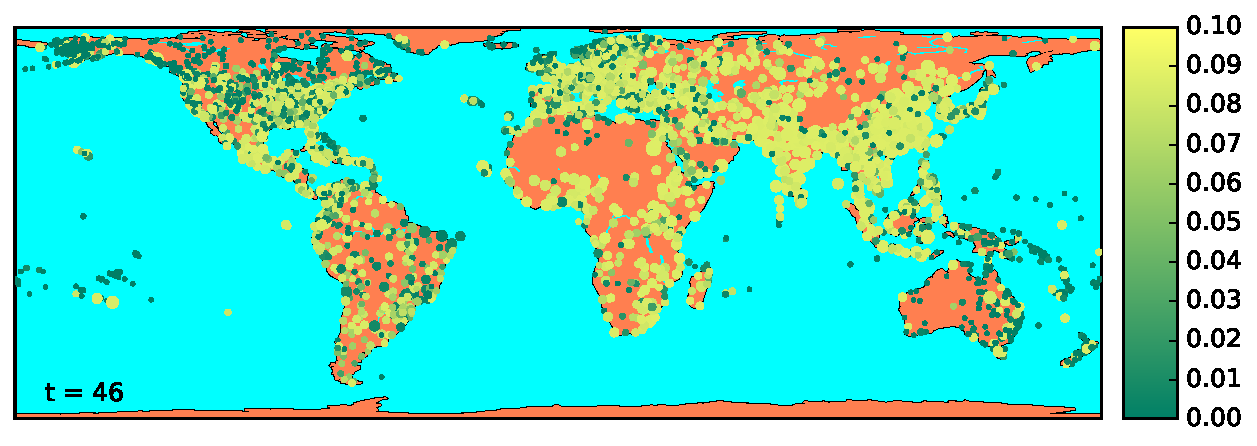
\includegraphics[width=1.0 \linewidth]{plots/gifs/frames/rio-46}
	\caption{Timestep 46, with Olympic Games. The full animation can be viewed at
		\url{https://andreasmadsen.github.io/course-02443-stochastic-virus-outbreaks/}}
	\label{fig:rio-46}
\end{figure}

\begin{figure}[H]
	\centering
	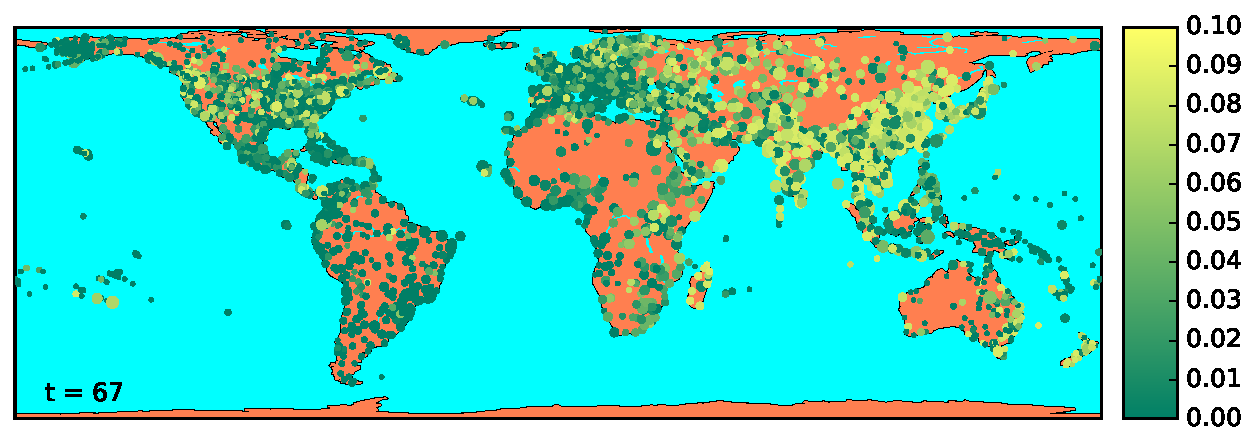
\includegraphics[width=1.0 \linewidth]{plots/gifs/frames/noRio-67}
	\caption{Timestep 67, without Olympic Games. The full animation can be viewed at
		\url{https://andreasmadsen.github.io/course-02443-stochastic-virus-outbreaks/}}
	\label{fig:noRio-67}
\end{figure}

From figure \ref{fig:rio-46} and figure \ref{fig:noRio-67} the conclusion from table \ref{table:olympic-summary} can be reconfirmed. The peak happens almost simultaneously across the globe when including the Olympic Games, while the spread pattern has a wave behaviour when not including the Olympic Games.
